\documentclass[a4paper,12pt]{report} % report, 12pt
\usepackage[utf8]{inputenc} % utf8
\usepackage{graphicx} % images
%\usepackage[pdf]{pstricks} %compilation pdf graphics
\usepackage[english]{babel}
\usepackage[T1]{fontenc} % accents

\usepackage{fancyhdr} %en-têtes et bas de page
\pagestyle{fancy}
\setlength{\headheight}{15pt}
\setlength{\footskip}{60pt} 

\usepackage{times} % Times New Roman

\usepackage{titlepic} %picture page garde

%%\usepackage{hyperref}% pour le \url

\title{Team Work Report in \LaTeX}
\titlepic{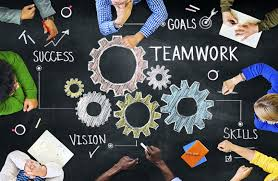
\includegraphics[width=0.7\textwidth]{teamwork.jpeg}}	 
\author{Grégoire MEUNIER}
\date{La date de rendu du rapport est le : \today}

%Definition des en-têtes
\fancyhead[L]{Grégoire Meunier}
\fancyhead[C]{\today}
\fancyhead[R]{Team Work Report}	

\fancyfoot[C]{\thepage}
\fancyfoot[R]{
\includegraphics[scale=0.2]{logo_utc.png}}
\fancyfoot[L]{
\includegraphics[scale=0.15]{logo_tuke.png}}

\renewcommand{\contentsname}{Contents Table}




%-----------------------------------------------------------------------------------BEGIN DOCUMENT---------------------------------%
\begin{document}
% --------------------------------------------------------------------PAGE DE GARDE------------------------------------------------%
\maketitle
% --------------------------------------------------------------------SOMMAIRE-----------------------------------------------------%
\tableofcontents

%--------------------------------------------------------FIRST CHAPTER-------------------------------------------------------------%
\chapter{What is Conflict Management ?}\newpage
Your goal is to makes the conflict happens the better you can. The final result of that conflict should be that every part of the conflict had clearly discribed what they wanted. Then we arrived in the situation that everyone’s wants and needs were respect during the process of resolution.
%------------------------------------------FIRST SECTION---------------------------------------------------------------------------%
\section{Different type of conflict management}
\subsection{Preventative measures}
It takes time to use this way, but it sure will be efficient.
\begin{itemize}
\item Workplace changes : Reorganise the framwork of the place.
\item Training staff : Know exactly what everybody has to do.
\item Conflict resolution policy : Give to your people access to training in communication.
\end{itemize}
\subsection{Alternative dispute resolution}
When basique methods doesn't get success, we need to go deeper in the problem. Make people talk with differents people in the way to find an arrangement.
\begin{itemize}
\item Informal discussions : Make people in the conflict talk together while you stay impartial. It gives people time to understand each other and to start again on a good basement.
\item Mediation : A third person that make people talk in a good environment in the way to solve problems. People calm down and find a good conclusion to fix the situation.
\item Conciliation : A third person who makes people talk and decide for them what they shloud do in order to fix the solution.
\item Arbitration : It is more official than previous methods. There is lawyers defending each person and an arbitrator to impose a legally-blinding settlement.
\end{itemize}
%----------------------------------------SECOND SECTION----------------------------------------------------------------------------%
\section{Causes of conflict at Work}
First of all, it is mostly because of several persons, and not because of just one of them. The goal here is to understand clearly what is the problem and act positively in order to prevent it from happening another time.
\subsection{Common causes of conflict at work}
\begin{itemize}
\item Differences in personality
\item Differences in styles of working
\item Miscommunication or misunderstandings
\item Availability of resources
\item Level of support
\item Poor customer service
\item Poorly-organised workplace
\item Poor management
\item Discrimination, harassment, etc.
\item Contract of employment
\end{itemize}
%---------------------------------------THIRD SECTION-----------------------------------------------------------------------------%
\section{Top Tips for Managing Conflict in the Workplace}
\begin{enumerate}
\item Do a conflict risk assessment
\item Don’t ignore it
\item Put in place an ‘open door’ policy
\item Promote differences
\item Become a mediator
\item Provide support and resources
\item Learn to listen actively
\item Stay calm and in control
\item Attack the problem, not the person
\item Be supportive
\end{enumerate}

%--------------------------------------------------------FIRST CHAPTER------------------------------------------------------------%
\chapter{Difference Between Group and Team}\newpage
When two or more individuals are classed together either by the organization or out of social needs, it is known as a group.
On the other hand, a team is the collection of people, who are linked together to achieve a common objective.
%-------------------------------------------FIRST SECTION-------------------------------------------------------------------------%
\section{Definition of Group}
\begin{itemize}
\item Un canard.
\item Un mammouth.
\end{itemize}
%------------------------------------------SECOND SECTION-------------------------------------------------------------------------%
\section{Definition of Team}
\begin{enumerate}
\item Hey
\end{enumerate}
%------------------------------------------THIRD SECTION--------------------------------------------------------------------------%
\section{Another}


\footnote{Texte de la note.}


\end{document}

